% Paper Narrative (literature-grounded, v2) for the NASA Space Apps 2026 entry "Sea Level Detective"
% Built from the paper-narrative skill template. Compile with pdflatex.
\documentclass[10pt]{article}
\usepackage{mathptmx}\usepackage[scaled=0.9]{helvet}\usepackage[T1]{fontenc}
\usepackage[landscape,margin=0.5in]{geometry}
\usepackage{amsmath,amssymb,enumitem,xcolor}
\usepackage{tikz}
\usetikzlibrary{arrows.meta,shapes.geometric}
\usepackage{microtype}
\renewcommand{\familydefault}{\sfdefault}
\setlist{nosep,leftmargin=1.4em}
\setlength{\parindent}{0pt}
\hyphenpenalty=10000 \exhyphenpenalty=10000 \emergencystretch=2em
\pagestyle{empty}

\newcommand{\NB}{5}
\newcommand{\colw}{5.08}
\newcommand{\beaty}{-1.45}
\newcommand{\evtop}{-3.75}
\newcommand{\evstep}{1.45}
\newcommand{\vy}{-9.35}
\newcommand{\beath}{2.25}

\tikzset{
  beatbox/.style={draw=black!70,line width=0.4pt,fill=white,inner sep=5pt,font=\small},
  claimbox/.style={beatbox,draw=black,line width=1.5pt,fill=black!9},
  evbase/.style={inner sep=0pt,font=\scriptsize\bfseries,line width=0.5pt},
  evL/.style={rectangle,minimum size=0.42cm},
  evT/.style={diamond,minimum size=0.60cm},
  evN/.style={circle,minimum size=0.47cm},
  stsolid/.style={fill=black,draw=black,text=white},
  stpartial/.style={fill=white,draw=black},
  stmissing/.style={fill=white,draw=black!55,text=black!55,dash pattern=on 1.5pt off 1.2pt},
  vbase/.style={font=\scriptsize\bfseries,align=center,inner sep=2pt,minimum height=0.5cm,line width=0.5pt,
                text width=\dimexpr\colw cm-0.80cm\relax},
  vsupported/.style={fill=black,draw=black,text=white},
  vthin/.style={fill=white,draw=black},
  vopen/.style={fill=white,draw=black!55,text=black!55,dash pattern=on 1.5pt off 1.2pt},
}
\newcommand{\beatbody}[2]{\parbox[t][\beath cm][t]{\dimexpr\colw cm-0.95cm\relax}{\raggedright #1\\[3pt]#2}}
\newcommand{\beat}[3]{\node[beatbox] (b#1) at ({(#1-0.5)*\colw},\beaty)
  {\beatbody{{\scriptsize\bfseries\color{black!60}#2}}{#3}};}
\newcommand{\claim}[3]{\node[claimbox] (b#1) at ({(#1-0.5)*\colw},\beaty)
  {\beatbody{{\scriptsize\bfseries #2}}{#3}};}
\newcommand{\spinearrows}{\foreach \i [evaluate=\i as \j using int(\i+1)] in {2,...,\NB}
  {\pgfmathtruncatemacro\p{\i-1}\draw[-{Latex[length=5pt]},line width=0.9pt] (b\p.east)--(b\i.west);}}
\newcommand{\stem}[2]{\pgfmathsetmacro\ex{(#1-1)*\colw+0.62}\pgfmathsetmacro\ey{\evtop-(#2-1)*\evstep}
  \draw[black!45,line width=0.5pt] (\ex,\ey) -- (\ex,\ey |- b#1.south);}
\newcommand{\ev}[6]{\pgfmathsetmacro\ex{(#1-1)*\colw+0.62}\pgfmathsetmacro\ey{\evtop-(#2-1)*\evstep}
  \node[evbase,ev#3,st#4] at (\ex,\ey) {#3};
  \node[anchor=west,align=left,font=\footnotesize,inner sep=0pt,text width=\dimexpr\colw cm-1.55cm\relax]
    at (\ex+0.42,\ey) {#5\\{\itshape\color{black!60}#6}};}
\newcommand{\verdict}[3]{\node[vbase,v#2] (v#1) at ({(#1-0.5)*\colw},\vy) {\MakeUppercase{#2}};
  \node[anchor=north,align=left,font=\scriptsize,inner sep=0pt,text width=\dimexpr\colw cm-0.80cm\relax]
    at ([yshift=-3pt]v#1.south) {#3};}
\newcommand{\mk}[2]{\tikz[baseline=-0.6ex]{\node[evbase,ev#1,st#2]{#1};}}

\begin{document}
{\LARGE\bfseries Narrative: Sea Level Detective}\hfill
{\small NASA Space Apps 2026, Trend Detective challenge \textperiodcentered{} literature-grounded \textperiodcentered{} status 2026-11-14}\\[3pt]
{\footnotesize Evidence:\enspace \mk{L}{solid} published literature / agency docs\quad \mk{T}{solid} deduction\quad
\mk{N}{solid} numerical (this project)\qquad
State:\enspace \mk{L}{solid} verified, says what the label says\quad \mk{L}{partial} read by co-reviewers only\quad
\mk{N}{missing} not yet built\qquad Heavy boxes are the key facts.}\\[-4pt]
\rule{\linewidth}{0.8pt}

\vspace{2pt}
{\small\textbf{In one breath:}\enspace
Short-record sea-level trends mix long-term rise with El Ni\~no swings of tens of centimetres that flip sign across the Pacific; so we
\textbf{remove the seasons and regress out a NASA ENSO index before an autocorrelation-aware trend test}, on \textbf{altimetry whose local
trends carry a published mean uncertainty of 0.83 mm/yr}, because \textbf{El Ni\~no is felt on U.S. coasts}, giving coastal communities
the local, El Ni\~no-aware trend they plan with.}
\vspace{6pt}

\noindent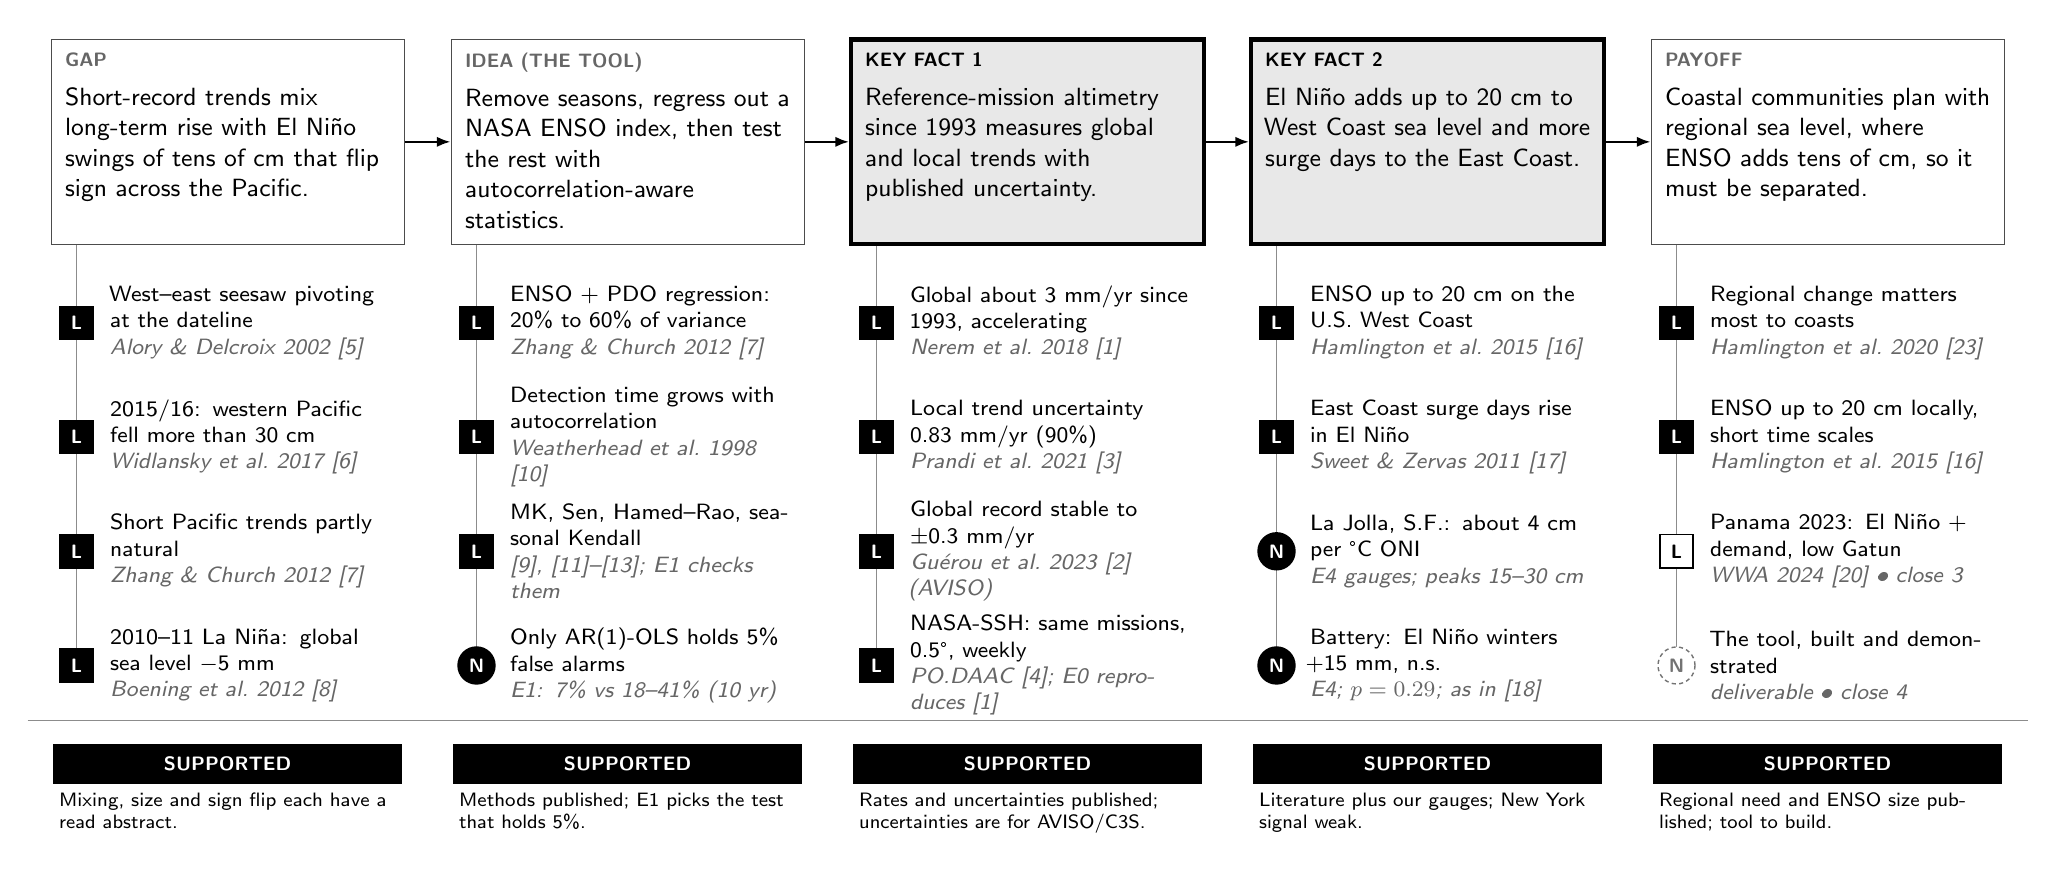
\begin{tikzpicture}[x=1cm,y=1cm]
\useasboundingbox (0,0) rectangle (25.4,{\vy-1.25});

\beat{1}{GAP}{Short-record trends mix long-term rise with El Ni\~no swings of tens of cm that flip sign across the Pacific.}
\beat{2}{IDEA (THE TOOL)}{Remove seasons, regress out a NASA ENSO index, then test the rest with autocorrelation-aware statistics.}
\claim{3}{KEY FACT 1}{Reference-mission altimetry since 1993 measures global and local trends with published uncertainty.}
\claim{4}{KEY FACT 2}{El Ni\~no adds up to 20 cm to West Coast sea level and more surge days to the East Coast.}
\beat{5}{PAYOFF}{Coastal communities plan with regional sea level, where ENSO adds tens of cm, so it must be separated.}
\spinearrows

\stem{1}{4}
\ev{1}{1}{L}{solid}{West--east seesaw pivoting at the dateline}{Alory \& Delcroix 2002 [5]}
\ev{1}{2}{L}{solid}{2015/16: western Pacific fell more than 30 cm}{Widlansky et al.\ 2017 [6]}
\ev{1}{3}{L}{solid}{Short Pacific trends partly natural}{Zhang \& Church 2012 [7]}
\ev{1}{4}{L}{solid}{2010--11 La Ni\~na: global sea level $-$5 mm}{Boening et al.\ 2012 [8]}

\stem{2}{4}
\ev{2}{1}{L}{solid}{ENSO + PDO regression: 20\% to 60\% of variance}{Zhang \& Church 2012 [7]}
\ev{2}{2}{L}{solid}{Detection time grows with autocorrelation}{Weatherhead et al.\ 1998 [10]}
\ev{2}{3}{L}{solid}{MK, Sen, Hamed--Rao, seasonal Kendall}{[9], [11]--[13]; E1 checks them}
\ev{2}{4}{N}{solid}{Only AR(1)-OLS holds 5\% false alarms}{E1: 7\% vs 18--41\% (10 yr)}

\stem{3}{4}
\ev{3}{1}{L}{solid}{Global about 3 mm/yr since 1993, accelerating}{Nerem et al.\ 2018 [1]}
\ev{3}{2}{L}{solid}{Local trend uncertainty 0.83 mm/yr (90\%)}{Prandi et al.\ 2021 [3]}
\ev{3}{3}{L}{solid}{Global record stable to $\pm$0.3 mm/yr}{Gu\'erou et al.\ 2023 [2] (AVISO)}
\ev{3}{4}{L}{solid}{NASA-SSH: same missions, 0.5\textdegree, weekly}{PO.DAAC [4]; E0 reproduces [1]}

\stem{4}{4}
\ev{4}{1}{L}{solid}{ENSO up to 20 cm on the U.S. West Coast}{Hamlington et al.\ 2015 [16]}
\ev{4}{2}{L}{solid}{East Coast surge days rise in El Ni\~no}{Sweet \& Zervas 2011 [17]}
\ev{4}{3}{N}{solid}{La Jolla, S.F.: about 4 cm per \textdegree C ONI}{E4 gauges; peaks 15--30 cm}
\ev{4}{4}{N}{solid}{Battery: El Ni\~no winters +15 mm, n.s.}{E4; $p = 0.29$; as in [18]}

\stem{5}{4}
\ev{5}{1}{L}{solid}{Regional change matters most to coasts}{Hamlington et al.\ 2020 [23]}
\ev{5}{2}{L}{solid}{ENSO up to 20 cm locally, short time scales}{Hamlington et al.\ 2015 [16]}
\ev{5}{3}{L}{partial}{Panama 2023: El Ni\~no + demand, low Gatun}{WWA 2024 [20] \textbullet{} close 3}
\ev{5}{4}{N}{missing}{The tool, built and demonstrated}{deliverable \textbullet{} close 4}

\draw[black!45,line width=0.4pt] (0,\vy+0.55) -- (25.4,\vy+0.55);
\verdict{1}{supported}{Mixing, size and sign flip each have a read abstract.}
\verdict{2}{supported}{Methods published; E1 picks the test that holds 5\%.}
\verdict{3}{supported}{Rates and uncertainties published; uncertainties are for AVISO/C3S.}
\verdict{4}{supported}{Literature plus our gauges; New York signal weak.}
\verdict{5}{supported}{Regional need and ENSO size published; tool to build.}
\end{tikzpicture}

\rule{\linewidth}{0.4pt}\\[3pt]
\begin{minipage}[t]{0.60\linewidth}\small
\textbf{To close, in order of damage to the story} (at most 4)
\begin{enumerate}[label=\textbf{\arabic*.}]
\item Set an Earthdata token and run E0--E3 so beats 1--3 gain our own NASA-SSH numbers next to the literature.
\item Rerun E1 with NASA box residuals (gauge noise is rougher than box means).
\item Read the WWA Panama report ourselves before the Panama panel goes on the site.
\item Build the tool and site on the E0--E4 outputs.
\end{enumerate}
\end{minipage}\hfill
\begin{minipage}[t]{0.36\linewidth}\small
\textbf{Scope of the claims}\\
The heavy boxes are facts the literature establishes; our own numbers come from E0--E8. The toggle regresses out the NASA ENSO index
only (decadal variability remains). East Coast and Panama are atmospheric links, not the ocean wave. Altimetry does not resolve harbors.
\end{minipage}
\end{document}
